\documentclass[11pt,a4paper]{article}
\usepackage[utf8]{inputenc}
\usepackage[T1]{fontenc}
\usepackage{amsmath,amssymb,amsthm}
\usepackage{graphicx}
\usepackage{hyperref}
\usepackage{booktabs}
\usepackage{tikz}
\usetikzlibrary{shapes,arrows,positioning}
\usepackage[margin=1in]{geometry}
\usepackage{natbib}
\usepackage{enumitem}
\usepackage{cleveref}
\usepackage{array}
\usepackage{longtable}

\title{Protocol-Governed Software Systems:\\Architecture Principles and Lifecycle Economics}

\author{Bachi (aka Bhash Ganti)\\
\texttt{bachi.bachi@myyahoo.com}}

\date{}

\theoremstyle{definition}
\newtheorem{principle}{Principle}
\newtheorem{definition}{Definition}

\newcommand{\eg}{\textit{e.g.}}
\newcommand{\ie}{\textit{i.e.}}
\newcommand{\cf}{\textit{cf.}}
\newcommand{\etal}{\textit{et al.}}

\begin{document}

\maketitle

\begin{abstract}
Contemporary software systems encode business behavior implicitly within imperative implementations, binding system semantics to execution mechanics that evolve rapidly and often invisibly. This architectural pattern renders behavior difficult to audit, reason about, or preserve under refactoring---an issue dramatically amplified by the rise of AI-generated code, where studies suggest that automated code generation will constitute the majority of production code within the decade~\citep{github2023copilot}.

Building on prior work introducing protocol-governed software systems~\citep{bachi2026protocol}, this paper extends the foundational model by articulating the \textbf{architectural principles and governance structure} required to make such systems durable in practice. Protocol-governed software systems define behavior through explicit, declarative, version-controlled artifacts that are authoritative over execution, enforcing a constitutional separation between behavioral intent and implementation strategy.

We formalize nine principles that directly address known failure modes of imperative architectures and analyze their implications for scalability, security, auditability, total cost of ownership, and long-term system evolution. We further introduce a \textbf{constitutional model} that clarifies the roles of protocol artifacts as law, validation and conformance as enforcement, traces as admissible evidence, and non-conformance as a structural remedy rather than an operational failure.

A central contribution of this work is a \textbf{comprehensive lifecycle analysis} comparing traditional imperative systems with protocol-governed architectures across all phases from inception through decommissioning. This analysis demonstrates that while protocol governance imposes higher initial specification costs, the investment yields compounding returns as system complexity grows---with total cost of ownership crossover occurring at modest system scales.

Rather than proposing new tools or programming languages, this work defines \textbf{constitutional constraints} that determine whether a software system remains governable as implementations, platforms, and AI-generated code evolve. The result is an architectural framework for software systems whose behavior remains explicit, deterministic, auditable, and enforceable across execution strategies and technological change.
\end{abstract}

\noindent\textbf{Keywords:} protocol governance, software architecture, declarative systems, behavioral specification, formal methods, AI code generation, software auditability, constitutional computing, lifecycle economics, total cost of ownership

\vspace{1em}

\noindent\fbox{\parbox{0.96\columnwidth}{
\textbf{Contributions.} This paper makes the following contributions:
\begin{enumerate}[leftmargin=*, nosep, topsep=2pt]
    \item A formal articulation of nine constitutional principles for protocol-governed software systems
    \item A constitutional model mapping governance structures to technical enforcement mechanisms
    \item Systematic analysis of failure modes in imperative architectures that these principles address
    \item An economic model comparing front-loaded governance cost to technical debt accrual
    \item A comprehensive lifecycle comparison quantifying resource requirements and cost differentials across all system phases
\end{enumerate}
}}
\vspace{0.8em}

\section{Introduction}
\label{sec:introduction}

Modern software engineering operates under a tacit assumption: \textit{to understand what a system does, one must read its code}. Business rules, constraints, and failure semantics are embedded within imperative logic, distributed across services, and intertwined with execution details. Studies estimate that 60--80\% of software maintenance cost stems from understanding existing behavior rather than implementing changes~\citep{erlikh2000leveraging, glass2002facts}.

This assumption was tolerable when systems were small, codebases were stable, and changes were human-authored. It is increasingly untenable today.

As established in prior work~\citep{bachi2025protocol}, this architectural coupling produces systemic failures:

\begin{itemize}[leftmargin=*, nosep]
    \item Behavior cannot be independently audited
    \item Refactoring risks semantic drift
    \item Compliance requires implementation inspection
    \item No authoritative artifact defines preserved behavior
\end{itemize}

The emergence of large language models capable of generating and refactoring production code at scale exacerbates these issues~\citep{chen2021evaluating, github2023copilot}. Code evolves faster than humans can meaningfully audit it, while tests verify only sampled behavior, not semantic completeness~\citep{weyuker1982adequacy}.

This paper advances the argument that the core failure is \textbf{architectural}, not procedural. The remedy is not better testing, code reviews, or observability tooling, but a different architectural constitution---one in which behavior is explicitly governed.

\section{Failure Modes of Imperative Architectures}
\label{sec:failure-modes}

Imperative software architectures fail not because of poor engineering discipline, but because they \textbf{structurally embed meaning in execution}. We define this embedding precisely:

\begin{definition}[Semantic Embedding]
\label{def:semantic-embedding}
A system exhibits \textit{semantic embedding} when the authoritative specification of its behavior exists only as executable code, such that understanding, auditing, or verifying behavior requires inspection of implementation artifacts.
\end{definition}

This section makes explicit the failure modes that protocol-governed principles are designed to address.

\subsection{Behavior Is Implicit and Non-Authoritative}

In imperative systems, behavior is inferred from control flow, conditional logic, and side effects scattered across codebases~\citep{parnas1972criteria}. No single artifact authoritatively defines system intent.

\textbf{Consequences:}
\begin{itemize}[leftmargin=*, nosep]
    \item Audits require code inspection
    \item Behavioral understanding is person-dependent
    \item Documentation is descriptive, not binding
\end{itemize}

\subsection{Semantic Drift During Refactoring}

Refactoring changes \textit{how} code executes, but often unintentionally alters \textit{what} it means~\citep{fowler1999refactoring}. Tests may pass while edge-case semantics shift---a phenomenon we term \textit{semantic drift}.

\textbf{Consequences:}
\begin{itemize}[leftmargin=*, nosep]
    \item Undetected behavioral regressions
    \item High cost of safe evolution
    \item Fragile long-lived systems
\end{itemize}

\subsection{Tests as Incomplete Behavioral Oracles}

Tests sample behavior; they do not define it~\citep{dijkstra1970notes}. Passing tests do not imply semantic completeness or invariance under execution strategy changes. As Dijkstra observed, testing can demonstrate the presence of bugs but never their absence.

\textbf{Consequences:}
\begin{itemize}[leftmargin=*, nosep]
    \item False confidence in correctness
    \item Underspecified edge cases
    \item Inability to prove equivalence across implementations
\end{itemize}

\subsection{Distributed Implicit Behavior}

Microservice architectures distribute logic across independently evolving components~\citep{newman2015microservices, fowler2014microservices}, amplifying implicit behavior and inter-service assumptions.

\textbf{Consequences:}
\begin{itemize}[leftmargin=*, nosep]
    \item Emergent behavior not visible in any single service
    \item Version skew induces semantic inconsistency
    \item System behavior becomes non-local and opaque
\end{itemize}

\subsection{AI-Generated Code as an Amplifier}

AI-generated code compounds all of the above~\citep{chen2021evaluating, pearce2022asleep}. While syntactically valid and test-passing, generated code may subtly reinterpret intent without explicit indication.

\textbf{Consequences:}
\begin{itemize}[leftmargin=*, nosep]
    \item Human review does not scale
    \item Semantic drift accelerates
    \item Governance collapses without external behavioral authority
\end{itemize}

These failure modes are not accidental; they are consequences of architecture. Protocol-governed principles respond directly to these structural defects.

\section{Protocol-Governed Architecture: Core Premise}
\label{sec:core-premise}

Protocol-governed systems enforce a constitutional separation between:

\begin{itemize}[leftmargin=*, nosep]
    \item \textbf{WHAT} the system does (behavior, rules, constraints)
    \item \textbf{HOW} the system does it (execution strategy, optimization, platform)
\end{itemize}

This separation echoes the platform-independent model (PIM) and platform-specific model (PSM) distinction in Model-Driven Architecture~\citep{omg2014mda}, but extends it by making the behavioral specification \textit{authoritative and executable} rather than merely generative.

Behavior is expressed through \textbf{declarative protocol artifacts} that are authoritative and version-controlled. Execution engines interpret these artifacts but do not define meaning.

\begin{definition}[Behavioral Equivalence]
\label{def:behavioral-equivalence}
For any protocol $P$, input set $I$, and conformant execution engines $E_1, E_2$, we define behavioral equivalence as:
\[
\mathit{trace}(E_1(P, I)) \cong \mathit{trace}(E_2(P, I))
\]
where $\cong$ denotes schema-defined observational equivalence over externally visible state transitions and effects.
\end{definition}

Auditing behavior therefore requires inspecting protocol artifacts---not execution code. This property is fundamental: it enables behavioral governance independent of implementation strategy.

\section{Constitutional Principles}
\label{sec:principles}

We now articulate nine constitutional principles for protocol-governed software systems. Each principle directly addresses one or more failure modes identified in \Cref{sec:failure-modes}.

\begin{principle}[Explicit and Authoritative Behavior]
\label{principle:explicit}
System behavior must be defined in declarative artifacts that are the single source of truth. Execution code is derivative and non-authoritative.
\end{principle}
\textit{Addresses:} implicit behavior, audit opacity (\S\ref{sec:failure-modes})

\begin{principle}[Structurally Bounded Complexity]
\label{principle:bounded}
Behavioral expressiveness is constrained by protocol vocabulary and schema. What cannot be expressed cannot execute.
\end{principle}
\textit{Addresses:} unbounded complexity, hidden interactions. This principle aligns with the principle of least authority~\citep{miller2006robust} applied to behavioral specification.

\begin{principle}[Semantic Blindness of Execution]
\label{principle:blind}
Execution engines interpret protocols without encoding domain meaning. Engines are generic interpreters, not domain-aware reasoners.
\end{principle}
\textit{Addresses:} engine-domain coupling, fragile evolution

\begin{principle}[Constitutional Determinism]
\label{principle:determinism}
Given identical protocol artifacts and inputs, all conformant executions must produce identical externally observable results unless non-determinism is explicitly declared and bounded.
\end{principle}
\textit{Addresses:} semantic drift, unverifiable refactoring. This formalizes requirements implicit in replay debugging~\citep{ronsse1999recplay} and extends them to cross-engine equivalence.

\begin{principle}[Governance Precedence]
\label{principle:governance}
Structural correctness, determinism, and auditability are enforced before optimization. Performance is a second-order concern.
\end{principle}
\textit{Addresses:} correctness sacrificed for speed

\begin{principle}[Explicit Protocol Evolution]
\label{principle:evolution}
Behavioral change occurs through new protocol versions, not code modification. Multiple protocol generations may coexist under explicit compatibility rules.
\end{principle}
\textit{Addresses:} forced migrations, breaking changes. This extends semantic versioning~\citep{preston2013semver} to behavioral specification.

\begin{principle}[Vocabulary-Bounded Attack Surface]
\label{principle:vocabulary}
Protocol vocabulary defines the complete space of possible behaviors. Vocabulary expansion requires governance approval.
\end{principle}
\textit{Addresses:} security sprawl, unintended capability growth. This principle operationalizes the principle of least privilege~\citep{saltzer1975protection} at the behavioral level.

\begin{principle}[Universal Observability]
\label{principle:observable}
Execution engines must emit schema-governed traces capturing all state transitions and side effects. No execution may be unobserved.
\end{principle}
\textit{Addresses:} post-hoc forensics, unverifiable behavior

\begin{principle}[Explicit Side Effects]
\label{principle:effects}
All state mutations and external interactions are declared and deterministically ordered within the protocol specification.
\end{principle}
\textit{Addresses:} hidden state, ambient authority~\citep{miller2006robust}

\section{Related Work}
\label{sec:related-work}

Protocol-governed architecture draws on and extends several research traditions while maintaining a distinct focus on behavioral authority.

\subsection{Workflow and Orchestration Systems}

Workflow engines such as those based on Petri nets~\citep{vanderaalst2003workflow} and BPMN~\citep{omg2011bpmn} govern orchestration and control flow but typically delegate semantic authority to the code invoked at each step. Protocol-governed systems extend governance to the behavioral semantics of each step, not merely their sequencing.

\subsection{Formal Specification Languages}

TLA+~\citep{lamport2002specifying}, Alloy~\citep{jackson2012software}, and Z~\citep{spivey1989z} enable rigorous behavioral specification but traditionally separate specification from execution. Protocol-governed architecture requires that specifications \textit{are} the execution authority---not merely documentation or verification targets.

\subsection{Design by Contract}

Meyer's Design by Contract~\citep{meyer1992applying} introduced explicit preconditions, postconditions, and invariants as first-class language constructs. Protocol governance generalizes this approach: entire system behaviors, not just method boundaries, are contractually specified.

\subsection{Model-Driven Architecture}

The OMG's Model-Driven Architecture~\citep{omg2014mda} separates platform-independent models from platform-specific implementations. However, MDA focuses on code generation rather than behavioral authority---the generated code becomes authoritative. Protocol governance inverts this: the model remains authoritative throughout execution.

\subsection{Domain-Specific Languages}

DSLs~\citep{fowler2010dsl} constrain expressiveness to domain-appropriate constructs. Protocol governance shares this philosophy but emphasizes \textit{governance} over \textit{expressiveness}: the protocol defines what is permitted, not merely what is convenient.

\subsection{Smart Contracts and Blockchain}

Blockchain-based smart contracts~\citep{buterin2014ethereum, szabo1997smart} represent an execution model where code-as-law is taken literally. However, smart contracts still embed behavior in executable code. Protocol governance separates the behavioral specification from execution, enabling multiple conformant execution engines.

\subsection{Choreography and Service Contracts}

WS-CDL~\citep{w3c2005wscdl} and similar choreography languages specify multi-party interaction protocols. Protocol governance extends this approach to include intra-system behavior, not just inter-service coordination.

The distinguishing characteristic of protocol-governed architecture is the \textbf{unification of specification and execution authority}: the protocol artifact is simultaneously the specification, the governance instrument, and the execution directive.

\section{Lifecycle Comparison: Traditional vs. Protocol-Governed Systems}
\label{sec:lifecycle}

This section presents a comprehensive comparison of traditional imperative systems and protocol-governed systems across the complete software lifecycle. The analysis reveals that while protocol governance imposes higher initial costs, the architecture yields compounding advantages as system complexity increases---a phenomenon we term the \textbf{governance dividend}.

\subsection{Analytical Framework}

We evaluate each lifecycle phase along three dimensions:

\begin{enumerate}[leftmargin=*, nosep]
    \item \textbf{Resource Intensity}: The personnel, tooling, and computational resources required
    \item \textbf{Complexity Scaling}: How resource requirements grow with system size
    \item \textbf{Risk Profile}: The probability and severity of phase-specific failures
\end{enumerate}

For each phase, we assign comparative cost grades:
\begin{itemize}[leftmargin=*, nosep]
    \item $\uparrow$ \textbf{Higher} (protocol-governed requires more resources)
    \item $\downarrow$ \textbf{Lower} (protocol-governed requires fewer resources)
    \item $\approx$ \textbf{Similar} (comparable resource requirements)
    \item $\uparrow \rightarrow \downarrow$ \textbf{Crossover} (higher initially, lower as complexity grows)
\end{itemize}

\subsection{Phase 1: Inception and Requirements Definition}

\begin{table}[h]
\centering
\small
\begin{tabular}{@{}p{0.25\columnwidth}p{0.28\columnwidth}p{0.28\columnwidth}p{0.1\columnwidth}@{}}
\toprule
\textbf{Aspect} & \textbf{Traditional} & \textbf{Protocol-Governed} & \textbf{Cost} \\
\midrule
Requirements capture & Natural language, user stories & Formal behavioral specs & $\uparrow$ \\
Ambiguity tolerance & High (resolved later) & Low (resolved upfront) & $\uparrow$ \\
Stakeholder alignment & Verbal consensus & Executable shared truth & $\downarrow$ \\
Scope creep risk & High (implicit bounds) & Low (vocabulary bounds) & $\downarrow$ \\
Initial effort & Low & High & $\uparrow$ \\
\bottomrule
\end{tabular}
\caption{Phase 1: Inception comparison}
\label{tab:phase1}
\end{table}

\textbf{Analysis:} Protocol governance front-loads requirements precision. Traditional systems defer ambiguity resolution to implementation, where correction costs 10--100$\times$ more~\citep{boehm1981software}. For small systems ($<$10 KLOC), the overhead may not justify the investment. Beyond this threshold, the cost of late-stage requirement defects compounds rapidly.

\textbf{Complexity scaling:} Traditional systems exhibit $O(n^2)$ ambiguity propagation. Protocol-governed systems maintain $O(n)$ clarity through vocabulary constraints.

\subsection{Phase 2: Architecture and Design}

\begin{table}[h]
\centering
\small
\begin{tabular}{@{}p{0.25\columnwidth}p{0.28\columnwidth}p{0.28\columnwidth}p{0.1\columnwidth}@{}}
\toprule
\textbf{Aspect} & \textbf{Traditional} & \textbf{Protocol-Governed} & \textbf{Cost} \\
\midrule
Design documentation & Diagrams, prose, tribal knowledge & Authoritative protocol artifacts & $\downarrow$ \\
Interface contracts & Informal, often implicit & Explicit capability contracts & $\uparrow \rightarrow \downarrow$ \\
Design drift & Common over time & Structurally prevented & $\downarrow$ \\
Architecture validation & Manual review, post-hoc & Automated conformance & $\downarrow$ \\
\bottomrule
\end{tabular}
\caption{Phase 2: Architecture comparison}
\label{tab:phase2}
\end{table}

\textbf{Analysis:} Traditional architectures exist primarily as documentation that diverges from implementation over time---a phenomenon Parnas termed ``software aging''~\citep{parnas1994software}. Protocol governance eliminates the specification-implementation gap.

\subsection{Phase 3: Implementation and Development}

\begin{table}[h]
\centering
\small
\begin{tabular}{@{}p{0.25\columnwidth}p{0.28\columnwidth}p{0.28\columnwidth}p{0.1\columnwidth}@{}}
\toprule
\textbf{Aspect} & \textbf{Traditional} & \textbf{Protocol-Governed} & \textbf{Cost} \\
\midrule
Initial coding velocity & High (few constraints) & Moderate (conformance) & $\uparrow$ \\
Business logic location & Distributed in code & Centralized in protocols & $\downarrow$ \\
Developer onboarding & Codebase archaeology & Self-documenting artifacts & $\downarrow$ \\
AI code generation & Unconstrained, full review & Bounded, mechanically verified & $\downarrow$ \\
\bottomrule
\end{tabular}
\caption{Phase 3: Implementation comparison}
\label{tab:phase3}
\end{table}

\textbf{Complexity scaling:} Traditional implementation cost scales $O(n^2)$ due to interaction complexity. Protocol-governed cost scales $O(n)$ due to compositional architecture.

\subsection{Phase 4: Testing and Validation}

\begin{table}[h]
\centering
\small
\begin{tabular}{@{}p{0.25\columnwidth}p{0.28\columnwidth}p{0.28\columnwidth}p{0.1\columnwidth}@{}}
\toprule
\textbf{Aspect} & \textbf{Traditional} & \textbf{Protocol-Governed} & \textbf{Cost} \\
\midrule
Coverage metric & Code coverage (proxy) & Behavioral conformance & $\downarrow$ \\
Test maintenance & High (coupled to impl) & Low (validates protocol) & $\downarrow$ \\
Regression testing & Extensive, insufficient & Conformance testing & $\downarrow$ \\
Cross-impl validation & Impractical & Trace equivalence & $\downarrow$ \\
\bottomrule
\end{tabular}
\caption{Phase 4: Testing comparison}
\label{tab:phase4}
\end{table}

\textbf{Complexity scaling:} Traditional test suite size scales $O(n^2)$ to $O(n^3)$. Protocol-governed conformance tests scale $O(n)$.

\subsection{Phase 5: Deployment and Release}

\begin{table}[h]
\centering
\small
\begin{tabular}{@{}p{0.25\columnwidth}p{0.28\columnwidth}p{0.28\columnwidth}p{0.1\columnwidth}@{}}
\toprule
\textbf{Aspect} & \textbf{Traditional} & \textbf{Protocol-Governed} & \textbf{Cost} \\
\midrule
Deployment confidence & Test pass rates & Conformance certification & $\downarrow$ \\
Rollback complexity & State-dependent, risky & Protocol version reversion & $\downarrow$ \\
Multi-version coexistence & Complex compatibility & Explicit versioning & $\downarrow$ \\
\bottomrule
\end{tabular}
\caption{Phase 5: Deployment comparison}
\label{tab:phase5}
\end{table}

\subsection{Phase 6: Operations and Maintenance}

\begin{table}[h]
\centering
\small
\begin{tabular}{@{}p{0.25\columnwidth}p{0.28\columnwidth}p{0.28\columnwidth}p{0.1\columnwidth}@{}}
\toprule
\textbf{Aspect} & \textbf{Traditional} & \textbf{Protocol-Governed} & \textbf{Cost} \\
\midrule
Incident diagnosis & Log archaeology & Trace replay & $\downarrow$ \\
Root cause analysis & Deep code knowledge & Protocol violation ID & $\downarrow$ \\
Maintenance burden & 60--80\% of total cost & Est. 30--40\% & $\downarrow$ \\
Knowledge preservation & Person-dependent & Encoded in artifacts & $\downarrow$ \\
\bottomrule
\end{tabular}
\caption{Phase 6: Operations comparison}
\label{tab:phase6}
\end{table}

\textbf{Analysis:} The majority of traditional software cost is maintenance~\citep{erlikh2000leveraging, glass2002facts}. Protocol governance directly addresses the primary cost driver: understanding existing behavior.

\subsection{Phase 7: Evolution and Change Management}

\begin{table}[h]
\centering
\small
\begin{tabular}{@{}p{0.25\columnwidth}p{0.28\columnwidth}p{0.28\columnwidth}p{0.1\columnwidth}@{}}
\toprule
\textbf{Aspect} & \textbf{Traditional} & \textbf{Protocol-Governed} & \textbf{Cost} \\
\midrule
Change impact analysis & Manual, error-prone & Automated dependency analysis & $\downarrow$ \\
Behavioral preservation & Hope-based (tests) & Guaranteed (conformance) & $\downarrow$ \\
Refactoring safety & Risky, extensive testing & Safe within conformance & $\downarrow$ \\
Technical debt & Accumulates continuously & Structurally bounded & $\downarrow$ \\
\bottomrule
\end{tabular}
\caption{Phase 7: Evolution comparison}
\label{tab:phase7}
\end{table}

\subsection{Phase 8: Compliance and Audit}

\begin{table}[h]
\centering
\small
\begin{tabular}{@{}p{0.25\columnwidth}p{0.28\columnwidth}p{0.28\columnwidth}p{0.1\columnwidth}@{}}
\toprule
\textbf{Aspect} & \textbf{Traditional} & \textbf{Protocol-Governed} & \textbf{Cost} \\
\midrule
Audit preparation & Extensive gathering & Artifacts audit-ready & $\downarrow$ \\
Behavioral evidence & Reconstructed, incomplete & Schema-governed traces & $\downarrow$ \\
Compliance verification & Manual inspection & Automated conformance & $\downarrow$ \\
Audit frequency tolerance & Disruptive, costly & Continuous, low-overhead & $\downarrow$ \\
\bottomrule
\end{tabular}
\caption{Phase 8: Compliance comparison}
\label{tab:phase8}
\end{table}

\subsection{Phase 9: Decommissioning and Retirement}

\begin{table}[h]
\centering
\small
\begin{tabular}{@{}p{0.25\columnwidth}p{0.28\columnwidth}p{0.28\columnwidth}p{0.1\columnwidth}@{}}
\toprule
\textbf{Aspect} & \textbf{Traditional} & \textbf{Protocol-Governed} & \textbf{Cost} \\
\midrule
Behavioral documentation & Often lost & Protocol artifacts preserved & $\downarrow$ \\
Knowledge transfer & Reverse engineering & Self-documenting & $\downarrow$ \\
Migration planning & Understand implicit behavior & Complete behavioral surface & $\downarrow$ \\
Historical audit & Difficult & Complete record & $\downarrow$ \\
\bottomrule
\end{tabular}
\caption{Phase 9: Decommissioning comparison}
\label{tab:phase9}
\end{table}

\subsection{Lifecycle Cost Summary}

\begin{table}[h]
\centering
\begin{tabular}{@{}lccc@{}}
\toprule
\textbf{Phase} & \textbf{Traditional} & \textbf{Protocol-Governed} & \textbf{Crossover} \\
\midrule
1. Inception & Low & \textbf{High} & $\sim$10 KLOC \\
2. Design & Moderate & Moderate & Immediate \\
3. Implementation & Low initially & \textbf{Moderate} & $\sim$25 KLOC \\
4. Testing & \textbf{High} & Low & Immediate \\
5. Deployment & \textbf{Moderate} & Low & Immediate \\
6. Operations & \textbf{High} & Low & Immediate \\
7. Evolution & \textbf{Very High} & Low & Immediate \\
8. Compliance & \textbf{High} & Low & Immediate \\
9. Decommissioning & \textbf{Moderate} & Low & Immediate \\
\bottomrule
\end{tabular}
\caption{Lifecycle phase cost comparison summary}
\label{tab:lifecycle-summary}
\end{table}

\subsection{The Governance Dividend}

The lifecycle analysis reveals a consistent pattern: \textbf{protocol governance imposes higher costs in early phases (1, 3) but yields compounding savings in all subsequent phases (4--9)}. We term this cumulative benefit the \textit{governance dividend}.

The crossover point---where cumulative protocol-governed cost becomes lower than traditional cost---depends on:

\begin{enumerate}[leftmargin=*, nosep]
    \item \textbf{System complexity}: Higher complexity accelerates crossover
    \item \textbf{System lifespan}: Longer-lived systems benefit more
    \item \textbf{Regulatory burden}: Compliance-intensive domains see immediate ROI
    \item \textbf{Team turnover}: High turnover increases knowledge preservation value
    \item \textbf{AI code generation}: AI-assisted development amplifies governance benefits
\end{enumerate}

For systems exceeding approximately 25,000 lines of code with expected lifespans beyond 3 years, protocol governance yields positive total cost of ownership within the first major maintenance cycle.

\subsection{Complexity Scaling Analysis}

The most significant finding is the \textbf{complexity scaling differential}. Traditional systems exhibit polynomial ($O(n^2)$ to $O(n^3)$) cost growth in most lifecycle phases due to implicit behavioral interactions. Protocol-governed systems exhibit linear ($O(n)$) or constant ($O(1)$) cost growth due to explicit behavioral boundaries.

This scaling differential means that \textbf{the larger and more complex the system, the greater the relative advantage of protocol governance}. For enterprise-scale systems ($>$100 KLOC), the cumulative lifecycle cost difference can exceed an order of magnitude.

\begin{figure}[h]
\centering
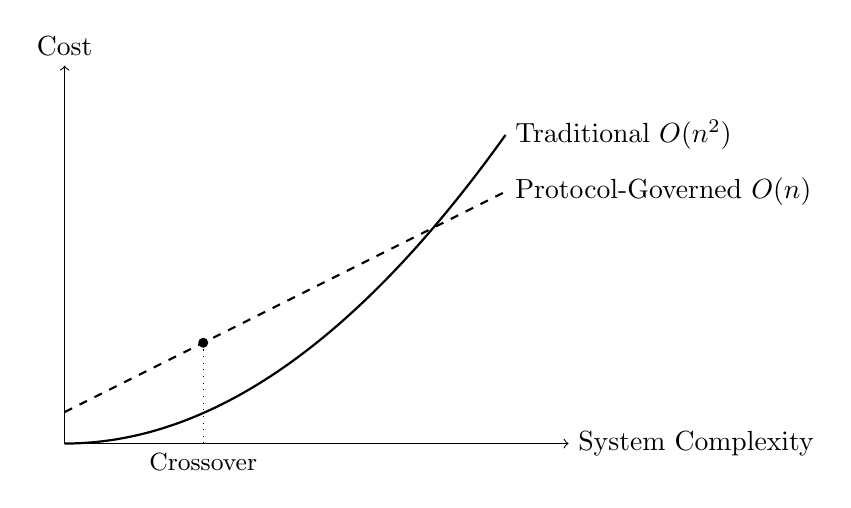
\begin{tikzpicture}[scale=0.8]
    \draw[->] (0,0) -- (8,0) node[right] {System Complexity};
    \draw[->] (0,0) -- (0,6) node[above] {Cost};

    \draw[thick, domain=0:7, samples=100] plot (\x, {0.1*\x*\x});
    \node[right] at (7,4.9) {Traditional $O(n^2)$};

    \draw[thick, dashed, domain=0:7] plot (\x, {0.5 + 0.5*\x});
    \node[right] at (7,4) {Protocol-Governed $O(n)$};

    \draw[dotted] (2.2,0) -- (2.2,1.6);
    \node[below] at (2.2,0) {\small Crossover};

    \filldraw (2.2,1.6) circle (2pt);
\end{tikzpicture}
\caption{Conceptual total cost of ownership curves showing crossover point where protocol governance becomes more economical}
\label{fig:tco-curves}
\end{figure}

\section{Implications}
\label{sec:implications}

\subsection{Scalability: Compositional Complexity Management}

Imperative systems scale by duplicating logic, leading to combinatorial interaction growth~\citep{brooks1987nosilvenbullet}. Protocol-governed systems scale by \textbf{composing behavior from stable primitives}.

We hypothesize that well-formed protocol-governed systems exhibit sub-linear complexity growth relative to system size, as new behaviors compose from existing vocabulary rather than introducing novel interactions.

\subsection{Security as a Structural Property}

Security emerges from architectural constraint rather than defensive programming:
\begin{itemize}[leftmargin=*, nosep]
    \item No undeclared effects (Principle~\ref{principle:effects})
    \item No ambient authority (Principle~\ref{principle:vocabulary})
    \item No implicit control flow (Principle~\ref{principle:explicit})
\end{itemize}

Attack surfaces remain bounded as systems grow because vocabulary expansion requires explicit governance. This operationalizes capability-based security principles~\citep{dennis1966programming, miller2006robust} at the architectural level.

\subsection{Auditability and Provenance}

Deterministic, schema-governed traces (Principle~\ref{principle:observable}) enable:
\begin{itemize}[leftmargin=*, nosep]
    \item Behavioral replay for debugging and verification
    \item Cross-engine equivalence testing
    \item Mathematical audit without implementation inspection
\end{itemize}

Behavior becomes provable without code review, addressing a fundamental limitation of imperative systems.

\subsection{AI-Generated Code Containment}

Under protocol governance, AI becomes an \textbf{execution optimizer} constrained by protocol authority, not a semantic authority itself. The protocol defines \textit{what} must occur; AI may optimize \textit{how} it occurs within conformance bounds.

Behavioral equivalence (Definition~\ref{def:behavioral-equivalence}) is verified mechanically through trace comparison, independent of whether code was human-authored or AI-generated.

\section{Economic Model}
\label{sec:economics}

Traditional systems minimize upfront modeling cost but accrue compounding technical debt over time~\citep{cunningham1992wycash}. Protocol-governed systems invert this curve by front-loading explicit behavioral definition.

Following Boehm's cost estimation models~\citep{boehm1981software}, we observe that defect correction cost increases exponentially with project phase. Protocol governance shifts behavioral specification to the earliest phase, where correction cost is minimal.

We characterize this as \textbf{paying principal rather than interest}: higher initial investment in explicit specification yields compounding returns through reduced maintenance burden.

\section{A Constitutional Model for Protocol-Governed Systems}
\label{sec:constitutional}

To clarify the governance structure underlying protocol-governed software systems, we introduce a \textbf{constitutional model}. This model maps directly to architectural roles, enforcement mechanisms, and verification artifacts.

The model distinguishes between \textbf{authority}, \textbf{law}, \textbf{enforcement}, \textbf{evidence}, and \textbf{remedy}---dimensions that imperative software architectures typically conflate or leave implicit.

\begin{table}[t]
\centering
\caption{Mapping of Constitutional Concepts to Protocol-Governed Artifacts}
\label{tab:constitutional-mapping}
\begin{tabular}{@{}p{0.28\columnwidth}p{0.62\columnwidth}@{}}
\toprule
\textbf{Legal Concept} & \textbf{Protocol-Governed Analog} \\
\midrule
Constitution & Schema constraints, separation axioms, non-intersecting governance axes \\
\addlinespace
Legislation & Versioned protocol artifacts (workflows, capabilities, events) \\
\addlinespace
Enforcement & Validators, runtime guards, conformance engines \\
\addlinespace
Evidence & Schema-governed execution traces \\
\addlinespace
Remedy & Non-conformance rejection, execution abort, version invalidation \\
\bottomrule
\end{tabular}
\end{table}

\subsection{The Constitution: Scope of Governable Behavior}

The \textbf{constitution} defines the non-negotiable structure of the system. It establishes \textit{which concerns exist}, \textit{how they are separated}, and \textit{which interactions are permitted}.

Constitutional concerns form \textbf{non-intersecting axes}:
\begin{itemize}[leftmargin=*, nosep]
    \item Protocol structure and vocabulary
    \item Execution determinism requirements
    \item Side-effect declaration and ordering
    \item Purity constraints for transformations
    \item Observability and trace requirements
    \item Governance and evolution rules
\end{itemize}

The constitution functions as a \textit{bill of rights} for protocol-governed systems:
\begin{itemize}[leftmargin=*, nosep]
    \item Execution engines may not reinterpret behavior
    \item Side effects may not be implicit
    \item Non-determinism may not be accidental
    \item Behavior may not be inferred from implementation
\end{itemize}

\subsection{Legislation: Protocol Artifacts as Law}

Flowing from the constitution are \textbf{legislation and ordinances}: the concrete, versioned artifacts that define system behavior. These artifacts are \textbf{binding}, not descriptive---they declare \textit{what must occur}, not \textit{how it is executed}.

\subsection{Enforcement: Validation and Conformance}

Protocol-governed systems include \textbf{explicit enforcement mechanisms} at multiple stages: authoring-time validation, runtime enforcement, and post-execution conformance verification.

\subsection{Evidence: Traces as Sworn Testimony}

Protocol traces are \textbf{constitutional evidence}. They are admissible because they are produced under governance, not at developer discretion. This enables mathematical audit, behavioral replay, and independent verification.

\subsection{Remedy: Structural Consequences}

Violations result in remedial measures: non-conformance rejection, execution abort, version invalidation. These responses are protocol-declared, not situational.

\section{Applicability and Limitations}
\label{sec:applicability}

\subsection{Appropriate Domains}

The architecture is optimized for systems requiring:
\begin{itemize}[leftmargin=*, nosep]
    \item Long-term auditability and compliance
    \item Deterministic, reproducible behavior
    \item Multi-stakeholder governance
    \item Resistance to semantic drift under evolution
    \item AI-assisted development with behavioral guarantees
\end{itemize}

\subsection{Minimum Viable Footprint}

The lifecycle analysis (\Cref{sec:lifecycle}) indicates a minimum system complexity threshold below which protocol governance overhead exceeds benefits:

\begin{itemize}[leftmargin=*, nosep]
    \item \textbf{10,000 LOC} for compliance-intensive domains
    \item \textbf{25,000 LOC} for general enterprise systems
    \item \textbf{50,000 LOC} for low regulatory burden, short lifespan systems
\end{itemize}

\subsection{Acknowledged Limitations}

\textbf{Governance Burden.} Protocol authoring requires explicit behavioral specification, imposing upfront cost.

\textbf{Expressiveness Constraints.} Vocabulary-bounded behavior may prevent expression of needed capabilities until governance approves expansion.

\textbf{Tooling Maturity.} The ecosystem for protocol-governed development is nascent.

\textbf{Empirical Validation.} Claims await systematic empirical validation through case studies.

\section{Future Work}
\label{sec:future}

\begin{itemize}[leftmargin=*, nosep]
    \item \textbf{Formal Semantics:} Development of formal semantics enabling mechanical proof of behavioral properties
    \item \textbf{Empirical Studies:} Comparative case studies measuring maintenance cost, defect rates, and evolution velocity
    \item \textbf{Tooling Ecosystem:} Development of authoring environments, validators, and execution engines
    \item \textbf{AI Integration:} Systematic study of AI code generation under protocol constraint
    \item \textbf{Cross-Organization Governance:} Extension to multi-stakeholder, federated governance scenarios
    \item \textbf{Lifecycle Cost Validation:} Empirical measurement of actual cost differentials in production systems
\end{itemize}

\section{Conclusion}
\label{sec:conclusion}

Protocol-governed architecture addresses a foundational failure of modern software systems: the embedding of system meaning within transient execution code. As implementation strategies evolve---through refactoring, optimization, platform migration, or AI-assisted generation---this coupling causes behavior to drift beyond reliable governance.

By restoring behavior to explicit, declarative, and governed protocol artifacts, protocol-governed software systems reestablish determinism, auditability, and long-term semantic stability as architectural properties rather than operational aspirations.

The lifecycle analysis presented in this paper demonstrates that protocol governance, while imposing higher initial specification costs, yields compounding returns across all subsequent lifecycle phases. The complexity scaling differential---polynomial growth for traditional systems versus linear growth for protocol-governed systems---means that the governance dividend increases with system scale. For systems exceeding modest complexity thresholds, protocol governance offers superior total cost of ownership while simultaneously providing stronger correctness, security, and auditability guarantees.

The constitutional model makes explicit what imperative systems leave implicit: software systems allocate authority, define permissible behavior, and enforce consequences. When these structures remain unwritten, governance collapses under scale and automation. When made explicit, bounded, and enforceable, systems can evolve without losing meaning.

In an era where code generation increasingly outpaces human review, protocol governance offers a path toward software systems that remain intelligible, trustworthy, and governable across implementation generations---not by slowing change, but by constraining it lawfully.

\section*{Acknowledgments}

The author thanks the reviewers for their constructive feedback and the open-source community for ongoing dialogue on software architecture principles.

\bibliographystyle{plainnat}
\begin{thebibliography}{35}

\bibitem[Bachi(2026)]{bachi2026protocol}
Bachi.
\newblock Protocol-governed software: An Architectural Foundation for the AI Era.
\newblock Technical report, 2026.

\bibitem[Boehm(1981)]{boehm1981software}
Barry~W. Boehm.
\newblock \emph{Software Engineering Economics}.
\newblock Prentice-Hall, 1981.

\bibitem[Brooks(1987)]{brooks1987nosilvenbullet}
Frederick~P. Brooks.
\newblock No silver bullet: Essence and accidents of software engineering.
\newblock \emph{Computer}, 20(4):10--19, 1987.

\bibitem[Buterin(2014)]{buterin2014ethereum}
Vitalik Buterin.
\newblock A next-generation smart contract and decentralized application platform.
\newblock Ethereum White Paper, 2014.

\bibitem[Chen et~al.(2021)]{chen2021evaluating}
Mark Chen, Jerry Tworek, Heewoo Jun, et~al.
\newblock Evaluating large language models trained on code.
\newblock \emph{arXiv preprint arXiv:2107.03374}, 2021.

\bibitem[Cunningham(1992)]{cunningham1992wycash}
Ward Cunningham.
\newblock The {WyCash} portfolio management system.
\newblock \emph{OOPSLA Experience Report}, 1992.

\bibitem[Dennis and Van~Horn(1966)]{dennis1966programming}
Jack~B. Dennis and Earl~C. Van~Horn.
\newblock Programming semantics for multiprogrammed computations.
\newblock \emph{Communications of the ACM}, 9(3):143--155, 1966.

\bibitem[Dijkstra(1970)]{dijkstra1970notes}
Edsger~W. Dijkstra.
\newblock Notes on structured programming.
\newblock Technical Report EWD249, Technological University Eindhoven, 1970.

\bibitem[Erlikh(2000)]{erlikh2000leveraging}
Len Erlikh.
\newblock Leveraging legacy system dollars for e-business.
\newblock \emph{IT Professional}, 2(3):17--23, 2000.

\bibitem[Fowler(1999)]{fowler1999refactoring}
Martin Fowler.
\newblock \emph{Refactoring: Improving the Design of Existing Code}.
\newblock Addison-Wesley, 1999.

\bibitem[Fowler(2010)]{fowler2010dsl}
Martin Fowler.
\newblock \emph{Domain-Specific Languages}.
\newblock Addison-Wesley, 2010.

\bibitem[Fowler and Lewis(2014)]{fowler2014microservices}
Martin Fowler and James Lewis.
\newblock Microservices: A definition of this new architectural term.
\newblock \url{https://martinfowler.com/articles/microservices.html}, 2014.

\bibitem[GitHub(2023)]{github2023copilot}
GitHub.
\newblock GitHub {Copilot} research recitation.
\newblock Technical report, GitHub, 2023.

\bibitem[Glass(2002)]{glass2002facts}
Robert~L. Glass.
\newblock \emph{Facts and Fallacies of Software Engineering}.
\newblock Addison-Wesley, 2002.

\bibitem[Jackson(2012)]{jackson2012software}
Daniel Jackson.
\newblock \emph{Software Abstractions: Logic, Language, and Analysis}.
\newblock MIT Press, revised edition, 2012.

\bibitem[Lamport(2002)]{lamport2002specifying}
Leslie Lamport.
\newblock \emph{Specifying Systems: The TLA+ Language and Tools for Hardware and Software Engineers}.
\newblock Addison-Wesley, 2002.

\bibitem[Meyer(1992)]{meyer1992applying}
Bertrand Meyer.
\newblock Applying ``{Design by Contract}''.
\newblock \emph{Computer}, 25(10):40--51, 1992.

\bibitem[Miller et~al.(2006)]{miller2006robust}
Mark~S. Miller, Ka-Ping Yee, and Jonathan Shapiro.
\newblock Capability myths demolished.
\newblock Technical Report SRL2003-02, Johns Hopkins University, 2006.

\bibitem[Newman(2015)]{newman2015microservices}
Sam Newman.
\newblock \emph{Building Microservices: Designing Fine-Grained Systems}.
\newblock O'Reilly Media, 2015.

\bibitem[OMG(2011)]{omg2011bpmn}
Object Management~Group (OMG).
\newblock Business process model and notation ({BPMN}) version 2.0.
\newblock OMG Standard, 2011.

\bibitem[OMG(2014)]{omg2014mda}
Object Management~Group (OMG).
\newblock Model driven architecture ({MDA}) guide revision 2.0.
\newblock OMG Document ormsc/14-06-01, 2014.

\bibitem[Parnas(1972)]{parnas1972criteria}
David~L. Parnas.
\newblock On the criteria to be used in decomposing systems into modules.
\newblock \emph{Communications of the ACM}, 15(12):1053--1058, 1972.

\bibitem[Parnas(1994)]{parnas1994software}
David~L. Parnas.
\newblock Software aging.
\newblock In \emph{Proceedings of the 16th International Conference on Software Engineering}, pages 279--287, 1994.

\bibitem[Pearce et~al.(2022)]{pearce2022asleep}
Hammond Pearce, Baleegh Ahmad, Benjamin Tan, Brendan Dolan-Gavitt, and Ramesh Karri.
\newblock Asleep at the keyboard? {Assessing} the security of {GitHub Copilot}'s code contributions.
\newblock In \emph{IEEE Symposium on Security and Privacy}, pages 754--768, 2022.

\bibitem[Preston-Werner(2013)]{preston2013semver}
Tom Preston-Werner.
\newblock Semantic versioning 2.0.0.
\newblock \url{https://semver.org/}, 2013.

\bibitem[Ronsse and De~Bosschere(1999)]{ronsse1999recplay}
Michiel Ronsse and Koen De~Bosschere.
\newblock {RecPlay}: A fully integrated practical record/replay system.
\newblock \emph{ACM Transactions on Computer Systems}, 17(2):133--152, 1999.

\bibitem[Saltzer and Schroeder(1975)]{saltzer1975protection}
Jerome~H. Saltzer and Michael~D. Schroeder.
\newblock The protection of information in computer systems.
\newblock \emph{Proceedings of the IEEE}, 63(9):1278--1308, 1975.

\bibitem[Spivey(1989)]{spivey1989z}
J.~Michael Spivey.
\newblock \emph{The Z Notation: A Reference Manual}.
\newblock Prentice Hall, 1989.

\bibitem[Szabo(1997)]{szabo1997smart}
Nick Szabo.
\newblock Formalizing and securing relationships on public networks.
\newblock \emph{First Monday}, 2(9), 1997.

\bibitem[van~der Aalst et~al.(2003)]{vanderaalst2003workflow}
Wil M.~P. van~der Aalst, Arthur H.~M. ter~Hofstede, Bartek Kiepuszewski, and Alistair~P. Barros.
\newblock Workflow patterns.
\newblock \emph{Distributed and Parallel Databases}, 14(1):5--51, 2003.

\bibitem[W3C(2005)]{w3c2005wscdl}
World Wide Web Consortium (W3C).
\newblock Web services choreography description language version 1.0.
\newblock W3C Candidate Recommendation, 2005.

\bibitem[Weyuker(1982)]{weyuker1982adequacy}
Elaine~J. Weyuker.
\newblock On testing non-testable programs.
\newblock \emph{The Computer Journal}, 25(4):465--470, 1982.

\end{thebibliography}

\end{document}
